\renewcommand{\captiontitle}{Overview of the \omeganet{} architecture}
\begin{figure*}
\begin{center}

\begin{tikzpicture}
\newcommand{\tw}{\textwidth}

\node [anchor=south west] (image) at (0,0) {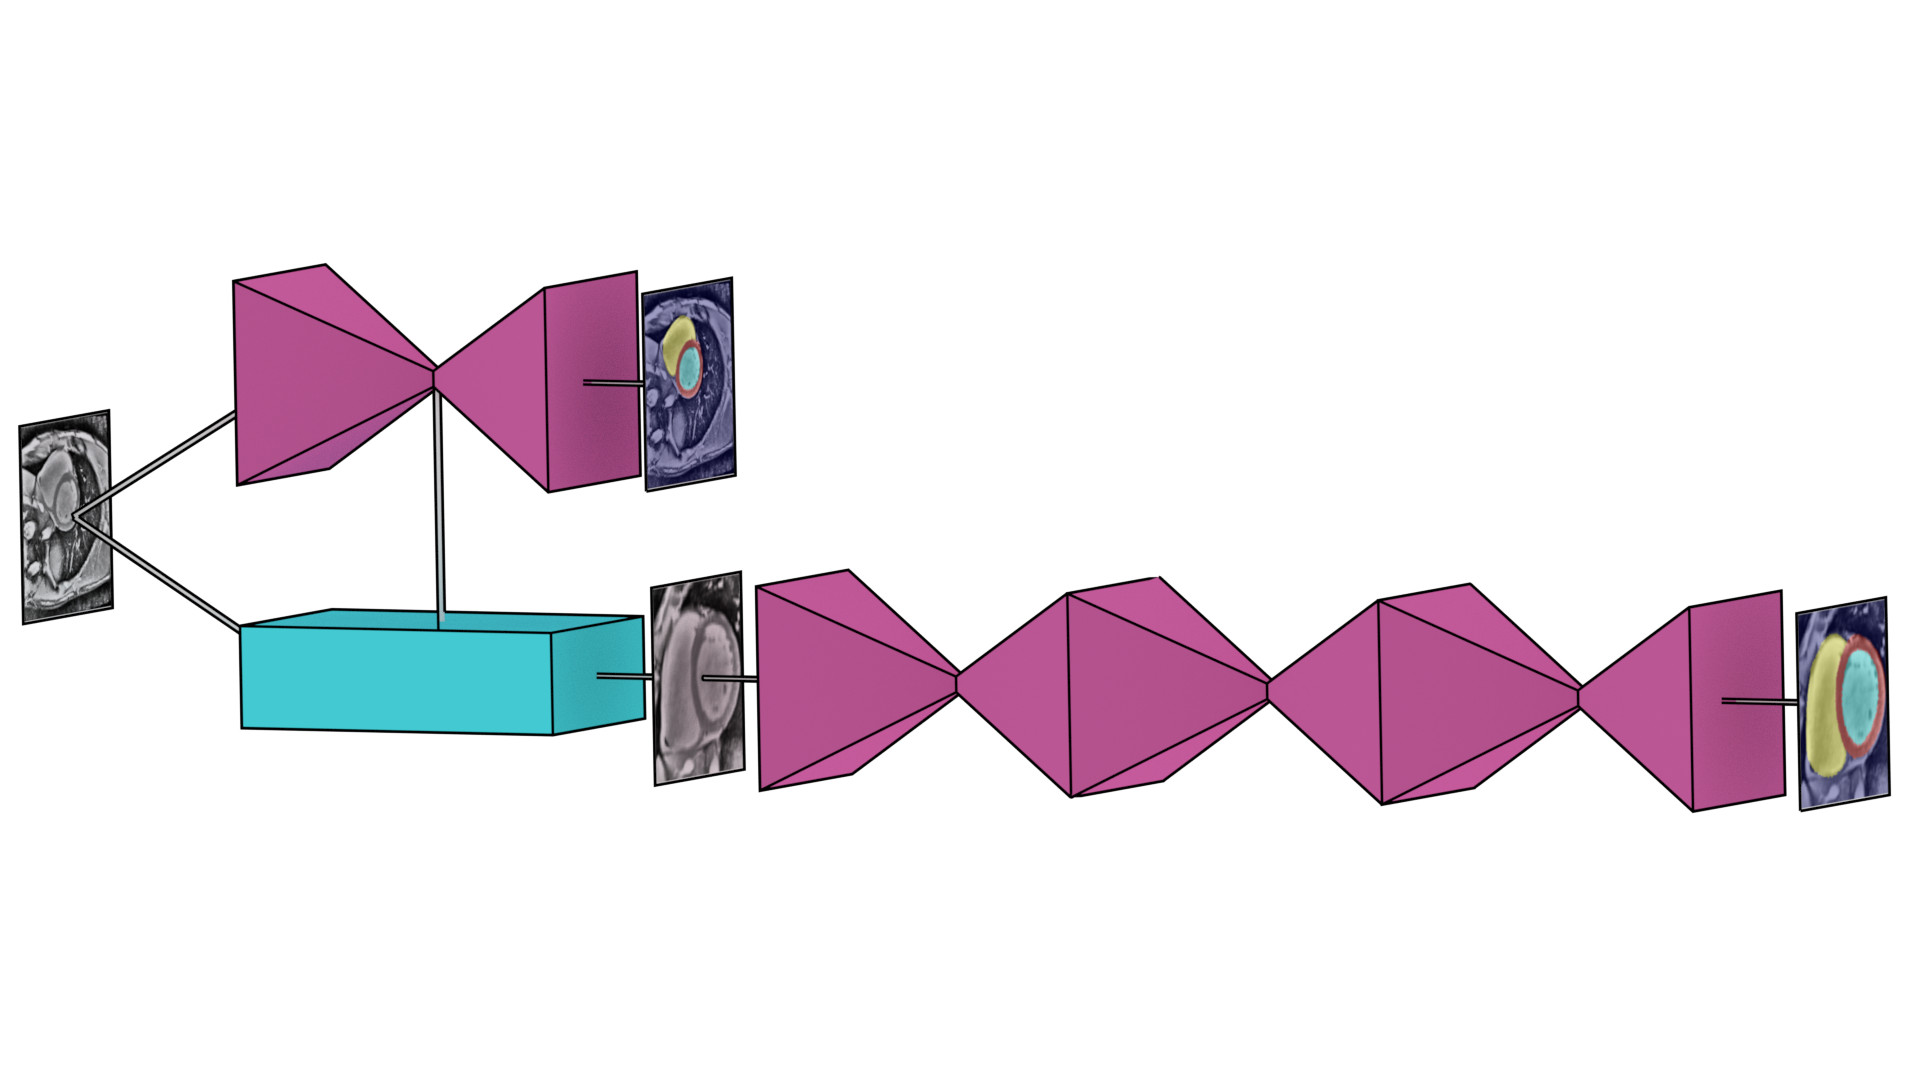
\includegraphics[clip, trim=0 260 0 260, width=1.0\textwidth]{./data/ohm-net-architecture.png}};

\node [anchor=south west] (a) at (0.025\tw,0.22\tw) {\large $\image$};
\node [anchor=south west] (b) at (0.35\tw,0.13\tw) {\large $\image^\prime$};
\node [anchor=south west] (c) at (0.35\tw,0.29\tw) {\large $S$};
\node [anchor=south west] (d) at (0.95\tw,0.13\tw) {\large $S^\prime$};
\node [anchor=south west] (e) at (0.17\tw,0.06\tw) {\large $\trans(\image, \tmat)$};

\draw [decorate,decoration={brace,amplitude=10pt},xshift=0pt,yshift=0pt](0.1275\tw,0.3\tw) -- (0.34\tw,0.3\tw) node [black,midway,xshift=0.0cm,yshift=+0.7cm] {(a) \hl{Initial} Segmentation Module};
\draw [decorate,decoration={brace,amplitude=10pt},xshift=0pt,yshift=0pt](0.3425\tw,0.045\tw) -- (0.1325\tw,0.045\tw) node [black,midway,xshift=0.0cm,yshift=-0.7cm] {(b) \hl{Transformation} Module};
\draw [decorate,decoration={brace,amplitude=10pt},xshift=0pt,yshift=0pt](0.4\tw,0.15\tw) -- (0.935\tw,0.15\tw) node [black,midway,xshift=0.0cm,yshift=+0.7cm] {(c) \hl{Final} Segmentation Module};
\end{tikzpicture}

\caption[\captiontitle]{\captiontitle{}.  (a) The initial, unoriented \SSFP{} image $\image$ is fed into a \UNet{} module, producing an \hl{initial} segmentation $S$.  (b) The features from the central (most downsampled) layers of this \UNet{} are used by the \hl{transformation} module to predict the parameters $\tmat$ of a rigid, affine transformation and transform the input image into a cannonical orientation, $\image^\prime = \trans(\image, \tmat)$.  (c) This transformed image is fed into a stacked hourglass module to obtain a \hl{final} segmentation in the canonical orientation $S^\prime$. Note that, all modules shown are trained in an end-to-end way from scratch.}
\label{fig:omega-net-architecture}
\end{center}
\end{figure*}
